\DeclareUnicodeCharacter{041B}{\CYRL}



\documentclass[11pt]{article}

    
    \usepackage{anyfontsize}
    \usepackage[breakable]{tcolorbox}
    \usepackage{parskip} % Stop auto-indenting (to mimic markdown behaviour)
    \usepackage[english,russian]{babel}
    \usepackage{graphicx}
    \usepackage{subcaption}

    % Basic figure setup, for now with no caption control since it's done
    % automatically by Pandoc (which extracts ![](path) syntax from Markdown).
    \usepackage{graphicx}
    % Maintain compatibility with old templates. Remove in nbconvert 6.0
    \let\Oldincludegraphics\includegraphics
    % Ensure that by default, figures have no caption (until we provide a
    % proper Figure object with a Caption API and a way to capture that
    % in the conversion process - todo).
    \usepackage{caption}

    \usepackage{float}
    \floatplacement{figure}{H} % forces figures to be placed at the correct location
    \usepackage{xcolor} % Allow colors to be defined
    \usepackage{enumerate} % Needed for markdown enumerations to work
    \usepackage{geometry} % Used to adjust the document margins
    \usepackage{amsmath} % Equations
    \usepackage{amssymb} % Equations
    \usepackage{textcomp} % defines textquotesingle
    % Hack from http://tex.stackexchange.com/a/47451/13684:
    \AtBeginDocument{%
        \def\PYZsq{\textquotesingle}% Upright quotes in Pygmentized code
    }
    \usepackage{upquote} % Upright quotes for verbatim code
    \usepackage{eurosym} % defines \euro

    \usepackage{iftex}
    \ifPDFTeX
        \usepackage[T1]{fontenc}
        \IfFileExists{alphabeta.sty}{
              \usepackage{alphabeta}
          }{
              \usepackage[mathletters]{ucs}
              \usepackage[utf8x]{inputenc}
          }
    \else
        \usepackage{fontspec}
        \usepackage{unicode-math}
    \fi

    \usepackage{fancyvrb} % verbatim replacement that allows latex
    \usepackage{grffile} % extends the file name processing of package graphics
                         % to support a larger range
    \makeatletter % fix for old versions of grffile with XeLaTeX
    \@ifpackagelater{grffile}{2019/11/01}
    {
      % Do nothing on new versions
    }
    {
      \def\Gread@@xetex#1{%
        \IfFileExists{"\Gin@base".bb}%
        {\Gread@eps{\Gin@base.bb}}%
        {\Gread@@xetex@aux#1}%
      }
    }
    \makeatother
    \usepackage[Export]{adjustbox} % Used to constrain images to a maximum size
    \adjustboxset{max size={0.9\linewidth}{0.9\paperheight}}

    % The hyperref package gives us a pdf with properly built
    % internal navigation ('pdf bookmarks' for the table of contents,
    % internal cross-reference links, web links for URLs, etc.)
    \usepackage{hyperref}
    % The default LaTeX title has an obnoxious amount of whitespace. By default,
    % titling removes some of it. It also provides customization options.
    \usepackage{titling}
    \usepackage{longtable} % longtable support required by pandoc >1.10
    \usepackage{booktabs}  % table support for pandoc > 1.12.2
    \usepackage{array}     % table support for pandoc >= 2.11.3
    \usepackage{calc}      % table minipage width calculation for pandoc >= 2.11.1
    \usepackage[inline]{enumitem} % IRkernel/repr support (it uses the enumerate* environment)
    \usepackage[normalem]{ulem} % ulem is needed to support strikethroughs (\sout)
                                % normalem makes italics be italics, not underlines
    \usepackage{mathrsfs}
    

    
    % Colors for the hyperref package
    \definecolor{urlcolor}{rgb}{0,.145,.698}
    \definecolor{linkcolor}{rgb}{.71,0.21,0.01}
    \definecolor{citecolor}{rgb}{.12,.54,.11}

    % ANSI colors
    \definecolor{ansi-black}{HTML}{3E424D}
    \definecolor{ansi-black-intense}{HTML}{282C36}
    \definecolor{ansi-red}{HTML}{E75C58}
    \definecolor{ansi-red-intense}{HTML}{B22B31}
    \definecolor{ansi-green}{HTML}{00A250}
    \definecolor{ansi-green-intense}{HTML}{007427}
    \definecolor{ansi-yellow}{HTML}{DDB62B}
    \definecolor{ansi-yellow-intense}{HTML}{B27D12}
    \definecolor{ansi-blue}{HTML}{208FFB}
    \definecolor{ansi-blue-intense}{HTML}{0065CA}
    \definecolor{ansi-magenta}{HTML}{D160C4}
    \definecolor{ansi-magenta-intense}{HTML}{A03196}
    \definecolor{ansi-cyan}{HTML}{60C6C8}
    \definecolor{ansi-cyan-intense}{HTML}{258F8F}
    \definecolor{ansi-white}{HTML}{C5C1B4}
    \definecolor{ansi-white-intense}{HTML}{A1A6B2}
    \definecolor{ansi-default-inverse-fg}{HTML}{FFFFFF}
    \definecolor{ansi-default-inverse-bg}{HTML}{000000}

    % common color for the border for error outputs.
    \definecolor{outerrorbackground}{HTML}{FFDFDF}

    % commands and environments needed by pandoc snippets
    % extracted from the output of `pandoc -s`
    \providecommand{\tightlist}{%
      \setlength{\itemsep}{0pt}\setlength{\parskip}{0pt}}
    \DefineVerbatimEnvironment{Highlighting}{Verbatim}{commandchars=\\\{\}}
    % Add ',fontsize=\small' for more characters per line
    \newenvironment{Shaded}{}{}
    \newcommand{\KeywordTok}[1]{\textcolor[rgb]{0.00,0.44,0.13}{\textbf{{#1}}}}
    \newcommand{\DataTypeTok}[1]{\textcolor[rgb]{0.56,0.13,0.00}{{#1}}}
    \newcommand{\DecValTok}[1]{\textcolor[rgb]{0.25,0.63,0.44}{{#1}}}
    \newcommand{\BaseNTok}[1]{\textcolor[rgb]{0.25,0.63,0.44}{{#1}}}
    \newcommand{\FloatTok}[1]{\textcolor[rgb]{0.25,0.63,0.44}{{#1}}}
    \newcommand{\CharTok}[1]{\textcolor[rgb]{0.25,0.44,0.63}{{#1}}}
    \newcommand{\StringTok}[1]{\textcolor[rgb]{0.25,0.44,0.63}{{#1}}}
    \newcommand{\CommentTok}[1]{\textcolor[rgb]{0.38,0.63,0.69}{\textit{{#1}}}}
    \newcommand{\OtherTok}[1]{\textcolor[rgb]{0.00,0.44,0.13}{{#1}}}
    \newcommand{\AlertTok}[1]{\textcolor[rgb]{1.00,0.00,0.00}{\textbf{{#1}}}}
    \newcommand{\FunctionTok}[1]{\textcolor[rgb]{0.02,0.16,0.49}{{#1}}}
    \newcommand{\RegionMarkerTok}[1]{{#1}}
    \newcommand{\ErrorTok}[1]{\textcolor[rgb]{1.00,0.00,0.00}{\textbf{{#1}}}}
    \newcommand{\NormalTok}[1]{{#1}}

    % Additional commands for more recent versions of Pandoc
    \newcommand{\ConstantTok}[1]{\textcolor[rgb]{0.53,0.00,0.00}{{#1}}}
    \newcommand{\SpecialCharTok}[1]{\textcolor[rgb]{0.25,0.44,0.63}{{#1}}}
    \newcommand{\VerbatimStringTok}[1]{\textcolor[rgb]{0.25,0.44,0.63}{{#1}}}
    \newcommand{\SpecialStringTok}[1]{\textcolor[rgb]{0.73,0.40,0.53}{{#1}}}
    \newcommand{\ImportTok}[1]{{#1}}
    \newcommand{\DocumentationTok}[1]{\textcolor[rgb]{0.73,0.13,0.13}{\textit{{#1}}}}
    \newcommand{\AnnotationTok}[1]{\textcolor[rgb]{0.38,0.63,0.69}{\textbf{\textit{{#1}}}}}
    \newcommand{\CommentVarTok}[1]{\textcolor[rgb]{0.38,0.63,0.69}{\textbf{\textit{{#1}}}}}
    \newcommand{\VariableTok}[1]{\textcolor[rgb]{0.10,0.09,0.49}{{#1}}}
    \newcommand{\ControlFlowTok}[1]{\textcolor[rgb]{0.00,0.44,0.13}{\textbf{{#1}}}}
    \newcommand{\OperatorTok}[1]{\textcolor[rgb]{0.40,0.40,0.40}{{#1}}}
    \newcommand{\BuiltInTok}[1]{{#1}}
    \newcommand{\ExtensionTok}[1]{{#1}}
    \newcommand{\PreprocessorTok}[1]{\textcolor[rgb]{0.74,0.48,0.00}{{#1}}}
    \newcommand{\AttributeTok}[1]{\textcolor[rgb]{0.49,0.56,0.16}{{#1}}}
    \newcommand{\InformationTok}[1]{\textcolor[rgb]{0.38,0.63,0.69}{\textbf{\textit{{#1}}}}}
    \newcommand{\WarningTok}[1]{\textcolor[rgb]{0.38,0.63,0.69}{\textbf{\textit{{#1}}}}}
    
% Pygments definitions
\makeatletter
\def\PY@reset{\let\PY@it=\relax \let\PY@bf=\relax%
    \let\PY@ul=\relax \let\PY@tc=\relax%
    \let\PY@bc=\relax \let\PY@ff=\relax}
\def\PY@tok#1{\csname PY@tok@#1\endcsname}
\def\PY@toks#1+{\ifx\relax#1\empty\else%
    \PY@tok{#1}\expandafter\PY@toks\fi}
\def\PY@do#1{\PY@bc{\PY@tc{\PY@ul{%
    \PY@it{\PY@bf{\PY@ff{#1}}}}}}}
\def\PY#1#2{\PY@reset\PY@toks#1+\relax+\PY@do{#2}}

\@namedef{PY@tok@w}{\def\PY@tc##1{\textcolor[rgb]{0.73,0.73,0.73}{##1}}}
\@namedef{PY@tok@c}{\let\PY@it=\textit\def\PY@tc##1{\textcolor[rgb]{0.24,0.48,0.48}{##1}}}
\@namedef{PY@tok@cp}{\def\PY@tc##1{\textcolor[rgb]{0.61,0.40,0.00}{##1}}}
\@namedef{PY@tok@k}{\let\PY@bf=\textbf\def\PY@tc##1{\textcolor[rgb]{0.00,0.50,0.00}{##1}}}
\@namedef{PY@tok@kp}{\def\PY@tc##1{\textcolor[rgb]{0.00,0.50,0.00}{##1}}}
\@namedef{PY@tok@kt}{\def\PY@tc##1{\textcolor[rgb]{0.69,0.00,0.25}{##1}}}
\@namedef{PY@tok@o}{\def\PY@tc##1{\textcolor[rgb]{0.40,0.40,0.40}{##1}}}
\@namedef{PY@tok@ow}{\let\PY@bf=\textbf\def\PY@tc##1{\textcolor[rgb]{0.67,0.13,1.00}{##1}}}
\@namedef{PY@tok@nb}{\def\PY@tc##1{\textcolor[rgb]{0.00,0.50,0.00}{##1}}}
\@namedef{PY@tok@nf}{\def\PY@tc##1{\textcolor[rgb]{0.00,0.00,1.00}{##1}}}
\@namedef{PY@tok@nc}{\let\PY@bf=\textbf\def\PY@tc##1{\textcolor[rgb]{0.00,0.00,1.00}{##1}}}
\@namedef{PY@tok@nn}{\let\PY@bf=\textbf\def\PY@tc##1{\textcolor[rgb]{0.00,0.00,1.00}{##1}}}
\@namedef{PY@tok@ne}{\let\PY@bf=\textbf\def\PY@tc##1{\textcolor[rgb]{0.80,0.25,0.22}{##1}}}
\@namedef{PY@tok@nv}{\def\PY@tc##1{\textcolor[rgb]{0.10,0.09,0.49}{##1}}}
\@namedef{PY@tok@no}{\def\PY@tc##1{\textcolor[rgb]{0.53,0.00,0.00}{##1}}}
\@namedef{PY@tok@nl}{\def\PY@tc##1{\textcolor[rgb]{0.46,0.46,0.00}{##1}}}
\@namedef{PY@tok@ni}{\let\PY@bf=\textbf\def\PY@tc##1{\textcolor[rgb]{0.44,0.44,0.44}{##1}}}
\@namedef{PY@tok@na}{\def\PY@tc##1{\textcolor[rgb]{0.41,0.47,0.13}{##1}}}
\@namedef{PY@tok@nt}{\let\PY@bf=\textbf\def\PY@tc##1{\textcolor[rgb]{0.00,0.50,0.00}{##1}}}
\@namedef{PY@tok@nd}{\def\PY@tc##1{\textcolor[rgb]{0.67,0.13,1.00}{##1}}}
\@namedef{PY@tok@s}{\def\PY@tc##1{\textcolor[rgb]{0.73,0.13,0.13}{##1}}}
\@namedef{PY@tok@sd}{\let\PY@it=\textit\def\PY@tc##1{\textcolor[rgb]{0.73,0.13,0.13}{##1}}}
\@namedef{PY@tok@si}{\let\PY@bf=\textbf\def\PY@tc##1{\textcolor[rgb]{0.64,0.35,0.47}{##1}}}
\@namedef{PY@tok@se}{\let\PY@bf=\textbf\def\PY@tc##1{\textcolor[rgb]{0.67,0.36,0.12}{##1}}}
\@namedef{PY@tok@sr}{\def\PY@tc##1{\textcolor[rgb]{0.64,0.35,0.47}{##1}}}
\@namedef{PY@tok@ss}{\def\PY@tc##1{\textcolor[rgb]{0.10,0.09,0.49}{##1}}}
\@namedef{PY@tok@sx}{\def\PY@tc##1{\textcolor[rgb]{0.00,0.50,0.00}{##1}}}
\@namedef{PY@tok@m}{\def\PY@tc##1{\textcolor[rgb]{0.40,0.40,0.40}{##1}}}
\@namedef{PY@tok@gh}{\let\PY@bf=\textbf\def\PY@tc##1{\textcolor[rgb]{0.00,0.00,0.50}{##1}}}
\@namedef{PY@tok@gu}{\let\PY@bf=\textbf\def\PY@tc##1{\textcolor[rgb]{0.50,0.00,0.50}{##1}}}
\@namedef{PY@tok@gd}{\def\PY@tc##1{\textcolor[rgb]{0.63,0.00,0.00}{##1}}}
\@namedef{PY@tok@gi}{\def\PY@tc##1{\textcolor[rgb]{0.00,0.52,0.00}{##1}}}
\@namedef{PY@tok@gr}{\def\PY@tc##1{\textcolor[rgb]{0.89,0.00,0.00}{##1}}}
\@namedef{PY@tok@ge}{\let\PY@it=\textit}
\@namedef{PY@tok@gs}{\let\PY@bf=\textbf}
\@namedef{PY@tok@gp}{\let\PY@bf=\textbf\def\PY@tc##1{\textcolor[rgb]{0.00,0.00,0.50}{##1}}}
\@namedef{PY@tok@go}{\def\PY@tc##1{\textcolor[rgb]{0.44,0.44,0.44}{##1}}}
\@namedef{PY@tok@gt}{\def\PY@tc##1{\textcolor[rgb]{0.00,0.27,0.87}{##1}}}
\@namedef{PY@tok@err}{\def\PY@bc##1{{\setlength{\fboxsep}{\string -\fboxrule}\fcolorbox[rgb]{1.00,0.00,0.00}{1,1,1}{\strut ##1}}}}
\@namedef{PY@tok@kc}{\let\PY@bf=\textbf\def\PY@tc##1{\textcolor[rgb]{0.00,0.50,0.00}{##1}}}
\@namedef{PY@tok@kd}{\let\PY@bf=\textbf\def\PY@tc##1{\textcolor[rgb]{0.00,0.50,0.00}{##1}}}
\@namedef{PY@tok@kn}{\let\PY@bf=\textbf\def\PY@tc##1{\textcolor[rgb]{0.00,0.50,0.00}{##1}}}
\@namedef{PY@tok@kr}{\let\PY@bf=\textbf\def\PY@tc##1{\textcolor[rgb]{0.00,0.50,0.00}{##1}}}
\@namedef{PY@tok@bp}{\def\PY@tc##1{\textcolor[rgb]{0.00,0.50,0.00}{##1}}}
\@namedef{PY@tok@fm}{\def\PY@tc##1{\textcolor[rgb]{0.00,0.00,1.00}{##1}}}
\@namedef{PY@tok@vc}{\def\PY@tc##1{\textcolor[rgb]{0.10,0.09,0.49}{##1}}}
\@namedef{PY@tok@vg}{\def\PY@tc##1{\textcolor[rgb]{0.10,0.09,0.49}{##1}}}
\@namedef{PY@tok@vi}{\def\PY@tc##1{\textcolor[rgb]{0.10,0.09,0.49}{##1}}}
\@namedef{PY@tok@vm}{\def\PY@tc##1{\textcolor[rgb]{0.10,0.09,0.49}{##1}}}
\@namedef{PY@tok@sa}{\def\PY@tc##1{\textcolor[rgb]{0.73,0.13,0.13}{##1}}}
\@namedef{PY@tok@sb}{\def\PY@tc##1{\textcolor[rgb]{0.73,0.13,0.13}{##1}}}
\@namedef{PY@tok@sc}{\def\PY@tc##1{\textcolor[rgb]{0.73,0.13,0.13}{##1}}}
\@namedef{PY@tok@dl}{\def\PY@tc##1{\textcolor[rgb]{0.73,0.13,0.13}{##1}}}
\@namedef{PY@tok@s2}{\def\PY@tc##1{\textcolor[rgb]{0.73,0.13,0.13}{##1}}}
\@namedef{PY@tok@sh}{\def\PY@tc##1{\textcolor[rgb]{0.73,0.13,0.13}{##1}}}
\@namedef{PY@tok@s1}{\def\PY@tc##1{\textcolor[rgb]{0.73,0.13,0.13}{##1}}}
\@namedef{PY@tok@mb}{\def\PY@tc##1{\textcolor[rgb]{0.40,0.40,0.40}{##1}}}
\@namedef{PY@tok@mf}{\def\PY@tc##1{\textcolor[rgb]{0.40,0.40,0.40}{##1}}}
\@namedef{PY@tok@mh}{\def\PY@tc##1{\textcolor[rgb]{0.40,0.40,0.40}{##1}}}
\@namedef{PY@tok@mi}{\def\PY@tc##1{\textcolor[rgb]{0.40,0.40,0.40}{##1}}}
\@namedef{PY@tok@il}{\def\PY@tc##1{\textcolor[rgb]{0.40,0.40,0.40}{##1}}}
\@namedef{PY@tok@mo}{\def\PY@tc##1{\textcolor[rgb]{0.40,0.40,0.40}{##1}}}
\@namedef{PY@tok@ch}{\let\PY@it=\textit\def\PY@tc##1{\textcolor[rgb]{0.24,0.48,0.48}{##1}}}
\@namedef{PY@tok@cm}{\let\PY@it=\textit\def\PY@tc##1{\textcolor[rgb]{0.24,0.48,0.48}{##1}}}
\@namedef{PY@tok@cpf}{\let\PY@it=\textit\def\PY@tc##1{\textcolor[rgb]{0.24,0.48,0.48}{##1}}}
\@namedef{PY@tok@c1}{\let\PY@it=\textit\def\PY@tc##1{\textcolor[rgb]{0.24,0.48,0.48}{##1}}}
\@namedef{PY@tok@cs}{\let\PY@it=\textit\def\PY@tc##1{\textcolor[rgb]{0.24,0.48,0.48}{##1}}}

\def\PYZbs{\char`\\}
\def\PYZus{\char`\_}
\def\PYZob{\char`\{}
\def\PYZcb{\char`\}}
\def\PYZca{\char`\^}
\def\PYZam{\char`\&}
\def\PYZlt{\char`\<}
\def\PYZgt{\char`\>}
\def\PYZsh{\char`\#}
\def\PYZpc{\char`\%}
\def\PYZdl{\char`\$}
\def\PYZhy{\char`\-}
\def\PYZsq{\char`\'}
\def\PYZdq{\char`\"}
\def\PYZti{\char`\~}
% for compatibility with earlier versions
\def\PYZat{@}
\def\PYZlb{[}
\def\PYZrb{]}
\makeatother


    % For linebreaks inside Verbatim environment from package fancyvrb.
    \makeatletter
        \newbox\Wrappedcontinuationbox
        \newbox\Wrappedvisiblespacebox
        \newcommand*\Wrappedvisiblespace {\textcolor{red}{\textvisiblespace}}
        \newcommand*\Wrappedcontinuationsymbol {\textcolor{red}{\llap{\tiny$\m@th\hookrightarrow$}}}
        \newcommand*\Wrappedcontinuationindent {3ex }
        \newcommand*\Wrappedafterbreak {\kern\Wrappedcontinuationindent\copy\Wrappedcontinuationbox}
        % Take advantage of the already applied Pygments mark-up to insert
        % potential linebreaks for TeX processing.
        %        {, <, #, %, $, ' and ": go to next line.
        %        _, }, ^, &, >, - and ~: stay at end of broken line.
        % Use of \textquotesingle for straight quote.
        \newcommand*\Wrappedbreaksatspecials {%
            \def\PYGZus{\discretionary{\char`\_}{\Wrappedafterbreak}{\char`\_}}%
            \def\PYGZob{\discretionary{}{\Wrappedafterbreak\char`\{}{\char`\{}}%
            \def\PYGZcb{\discretionary{\char`\}}{\Wrappedafterbreak}{\char`\}}}%
            \def\PYGZca{\discretionary{\char`\^}{\Wrappedafterbreak}{\char`\^}}%
            \def\PYGZam{\discretionary{\char`\&}{\Wrappedafterbreak}{\char`\&}}%
            \def\PYGZlt{\discretionary{}{\Wrappedafterbreak\char`\<}{\char`\<}}%
            \def\PYGZgt{\discretionary{\char`\>}{\Wrappedafterbreak}{\char`\>}}%
            \def\PYGZsh{\discretionary{}{\Wrappedafterbreak\char`\#}{\char`\#}}%
            \def\PYGZpc{\discretionary{}{\Wrappedafterbreak\char`\%}{\char`\%}}%
            \def\PYGZdl{\discretionary{}{\Wrappedafterbreak\char`\$}{\char`\$}}%
            \def\PYGZhy{\discretionary{\char`\-}{\Wrappedafterbreak}{\char`\-}}%
            \def\PYGZsq{\discretionary{}{\Wrappedafterbreak\textquotesingle}{\textquotesingle}}%
            \def\PYGZdq{\discretionary{}{\Wrappedafterbreak\char`\"}{\char`\"}}%
            \def\PYGZti{\discretionary{\char`\~}{\Wrappedafterbreak}{\char`\~}}%
        }
        % Some characters . , ; ? ! / are not pygmentized.
        % This macro makes them "active" and they will insert potential linebreaks
        \newcommand*\Wrappedbreaksatpunct {%
            \lccode`\~`\.\lowercase{\def~}{\discretionary{\hbox{\char`\.}}{\Wrappedafterbreak}{\hbox{\char`\.}}}%
            \lccode`\~`\,\lowercase{\def~}{\discretionary{\hbox{\char`\,}}{\Wrappedafterbreak}{\hbox{\char`\,}}}%
            \lccode`\~`\;\lowercase{\def~}{\discretionary{\hbox{\char`\;}}{\Wrappedafterbreak}{\hbox{\char`\;}}}%
            \lccode`\~`\:\lowercase{\def~}{\discretionary{\hbox{\char`\:}}{\Wrappedafterbreak}{\hbox{\char`\:}}}%
            \lccode`\~`\?\lowercase{\def~}{\discretionary{\hbox{\char`\?}}{\Wrappedafterbreak}{\hbox{\char`\?}}}%
            \lccode`\~`\!\lowercase{\def~}{\discretionary{\hbox{\char`\!}}{\Wrappedafterbreak}{\hbox{\char`\!}}}%
            \lccode`\~`\/\lowercase{\def~}{\discretionary{\hbox{\char`\/}}{\Wrappedafterbreak}{\hbox{\char`\/}}}%
            \catcode`\.\active
            \catcode`\,\active
            \catcode`\;\active
            \catcode`\:\active
            \catcode`\?\active
            \catcode`\!\active
            \catcode`\/\active
            \lccode`\~`\~
        }
    \makeatother

    \let\OriginalVerbatim=\Verbatim
    \makeatletter
    \renewcommand{\Verbatim}[1][1]{%
        %\parskip\z@skip
        \sbox\Wrappedcontinuationbox {\Wrappedcontinuationsymbol}%
        \sbox\Wrappedvisiblespacebox {\FV@SetupFont\Wrappedvisiblespace}%
        \def\FancyVerbFormatLine ##1{\hsize\linewidth
            \vtop{\raggedright\hyphenpenalty\z@\exhyphenpenalty\z@
                \doublehyphendemerits\z@\finalhyphendemerits\z@
                \strut ##1\strut}%
        }%
        % If the linebreak is at a space, the latter will be displayed as visible
        % space at end of first line, and a continuation symbol starts next line.
        % Stretch/shrink are however usually zero for typewriter font.
        \def\FV@Space {%
            \nobreak\hskip\z@ plus\fontdimen3\font minus\fontdimen4\font
            \discretionary{\copy\Wrappedvisiblespacebox}{\Wrappedafterbreak}
            {\kern\fontdimen2\font}%
        }%

        % Allow breaks at special characters using \PYG... macros.
        \Wrappedbreaksatspecials
        % Breaks at punctuation characters . , ; ? ! and / need catcode=\active
        \OriginalVerbatim[#1,codes*=\Wrappedbreaksatpunct]%
    }
    \makeatother

    % Exact colors from NB
    \definecolor{incolor}{HTML}{303F9F}
    \definecolor{outcolor}{HTML}{D84315}
    \definecolor{cellborder}{HTML}{CFCFCF}
    \definecolor{cellbackground}{HTML}{F7F7F7}

    % prompt
    \makeatletter
    \newcommand{\boxspacing}{\kern\kvtcb@left@rule\kern\kvtcb@boxsep}
    \makeatother
    \newcommand{\prompt}[4]{
        {\ttfamily\llap{{\color{#2}[#3]:\hspace{3pt}#4}}\vspace{-\baselineskip}}
    }
    

    
    % Prevent overflowing lines due to hard-to-break entities
    \sloppy
    % Setup hyperref package
    \hypersetup{
      breaklinks=true,  % so long urls are correctly broken across lines
      colorlinks=true,
      urlcolor=urlcolor,
      linkcolor=linkcolor,
      citecolor=citecolor,
      }
    % Slightly bigger margins than the latex defaults
    
    \geometry{verbose,tmargin=1in,bmargin=1in,lmargin=1in,rmargin=1in}
    
    

\begin{document}

    \begin{titlepage}
    \newpage
    
    \begin{center}
    МИНИСТЕРСТВО ОБРАЗОВАНИЯ РЕСПУБЛИКИ БЕЛАРУСЬ БЕЛОРУССКИЙ ГОСУДАРСТВЕННЫЙ УНИВЕРСИТЕТ \\
    Факультет прикладной математики и информатики \\ Кафедра компьютерных технологий и систем
    \end{center}
    
    \vspace{8em}
    
    \vspace{2em}
    
    \begin{center}
    \textsc{\textbf{Отчет по лабораторной работе 1
    \linebreak Вариант 5}}
    \end{center}
    
    \vspace{6em}
    
    \begin{flushright}
        Выполнил:\\
        Карпович Артём Дмитриевич\\
        студент 4 курса 7 группы
    \end{flushright}

    \begin{flushright}
        Преподаватель:\\
        Каркоцкий Александр Геннадьевич
    \end{flushright}
    \vspace{\fill}
    
    \begin{center}
    Минск, 2024
    \end{center}
    
    \end{titlepage}

\begin{center}
    \section*{Условие}
\end{center}
Решить следующие смешанные задачи методом разделения переменных. Произвести
визуализацию с использованием пакета Wolfram Mathematica. Первая задача посвящена
колебанию тонкой струны, вторая – прямоугольного контура. Сумма, при необходимости,
должна состоять не менее чем из 100 слагаемых.
\begin{enumerate}
    \item$$
        \begin{cases}
            u_{tt}-u_{xx}=x(2+t),0 < x < 5, t>0\\
            u|_{t=0}=x,\\
            u_t|_{t=0}=0,\\
            u_x+5u|_{x=0} = 1-t,\\
            u|_{x=5}=t.\\
        \end{cases}$$
    \item$$
        \begin{cases}
            u_{tt}=\Delta u,\\
            u|_{x=0}=u_x|_{x=5}=0,\\
            u_y|_{y=0}=u|_{y=9}=0,\\
            u|_{t=0} = e^{x+y},\\
            u_t|_{t=0}=e^{x-y}.\\
        \end{cases}$$
\end{enumerate}
\newpage
\section*{Задача 1}
\subsubsection*{Получение решения}
Перепишем условие задачи:
$$\begin{cases}
    u_{tt}-u_{xx}=x(2+t),0 < x < 5, t>0\\
    u|_{t=0}=x,\\
    u_t|_{t=0}=0,\\
    u_x+5u|_{x=0} = 1-t,\\
    u|_{x=5}=t.\\
\end{cases}$$
Решение задачи будем искать в виде суммы $$u(x,t)=v(x,t)+w(x,t),$$ где функция $v(x,t)$ удовлетворяет смешанной задаче с однородными граничными условиями, а функция $w(x,t)$ - неоднородным граничным условиям.

Найдем функцию $w(x,t)$ из представления:
$$w(x,t)=a(t)x^2+b(t)x+c(t).$$

Подставим это представление в граничные условия:
$$w_x(0,t)+5w(0,t)=b+5c=1-t,$$
$$w(5,t)=25a+5b+c=t.$$
Положим $a(t)=0$, тогда получим систему для $b, c$:
\begin{center}$
    \begin{cases}
        b+5c=1-t,\\
        5b+c=t.\\
    \end{cases} \Rightarrow 
    \begin{cases}
        b=\frac{1}{4}(t-\frac{1}{6}),\\
        c=\frac{1}{4}(\frac{5}{6}-t).\\
    \end{cases} \Rightarrow
    \omega = \frac{1}{4}(t-\frac{1}{6})x+\frac{1}{4}(\frac{5}{6}-t).
$\end{center}
Тогда решение исходной задачи представимо в виде:
$$u(x,t)=v(x,t)+\frac{1}{4}(t-\frac{1}{6})x+\frac{1}{4}(\frac{5}{6}-t).$$
Путём подстановки данного представления в исходную задачу получим задачу для $v(x,t)$ с однородными граничными условиями:
$$
        \begin{cases}
            v_{tt}-v_{xx}=x(2+t),\\
            v|_{t=0}=\frac{5}{24}(5x-1),\\
            v_t|_{t=0}=\frac{1}{4}(1-x),\\
            v_x+5v|_{x=0} = 0,\\
            v|_{x=5}=0.\\
        \end{cases}$$
Решение данной задачи будем искать в виде суммы:
$$v(x,t)=\sum^\infty_{k=0}X_k(x)T_k(t).$$
Составим задачу Штурма-Лиувилля для однородного уравнения:
$$\begin{cases}
    X''(x)+\lambda_k^2 X(x)=0,\\
    X'(0)+5X(0)=0,\\
    X(5)=0.\\
\end{cases}$$
Найдем общее решение уравнения данной задачи:
$$X_k(x)=A_kcos\lambda_kx+B_ksin\lambda_kx,$$
подставляем в граничные условия для нахождения коэффициентов:
$$\begin{cases}
    \lambda_kB_k+5A_k=0,\\
    A_kcos5\lambda_k+B_ksin5\lambda_k=0.\\
\end{cases}$$
Выразим из первого уравнения $A_k$: $$A_k = -\frac{\lambda_k}{5}B_k,$$ тогда, подставляя полученное во второе начальное условие, получим: $$-\frac{\lambda_k}{5}B_k\cos{5\lambda_k}+B_k\sin{5\lambda_k}=0, \Rightarrow (-\frac{\lambda_k}{5}\cos{5\lambda_k}+\sin{5\lambda_k})B_k=0$$ поскольку из выражения для $A_k$ следует, что $B_k \neq 0$ (в противном случае получаем нулевое решение), то можем разделить уравнение на $B_k$ и получим: $$\sin{5\lambda_k}=\frac{\lambda_k}{5}\cos{5\lambda_k} \Rightarrow \tg{5\lambda_k}=\frac{\lambda_k}{5}.$$ 
Положим $B=1$, тогда собственные функции задачи Штурма-Лиувилля примут вид: $$X_k(x)=\sin{\lambda_k x}-\frac{\lambda_k}{5}\cos{\lambda_k x}.$$
Собственные значения найдем чуть позже, при визуализации полученного решения, используя Wolfram Mathematica.
Таким образом, решение рассматриваемой задачи можно представить в виде:
$$v(x,t)=\sum^\infty_{k=0}(\sin{\lambda_k x}-\frac{\lambda_k}{5}\cos{\lambda_k x})T_k(t).$$
Подставим полученное представление в исходное уравнение и начальные условия рассматриваемой задачи:
$$\begin{cases}
    \sum^\infty_{k=0}(\sin{\lambda_k x}-\frac{\lambda_k}{5}\cos{\lambda_k x})(T_k''(t)+\lambda_k^2 T_k(t))=\sum^\infty_{k=0}(\sin{\lambda_k x}-\frac{\lambda_k}{5}\cos{\lambda_k x})f_k,\\
    \sum^\infty_{k=0}(\sin{\lambda_k x}-\frac{\lambda_k}{5}\cos{\lambda_k x})T_k(0)=\sum^\infty_{k=0}(\sin{\lambda_k x}-\frac{\lambda_k}{5}\cos{\lambda_k x})\varphi_k,\\
    \sum^\infty_{k=0}(\sin{\lambda_k x}-\frac{\lambda_k}{5}\cos{\lambda_k x})T_k'(0)=\sum^\infty_{k=0}(\sin{\lambda_k x}-\frac{\lambda_k}{5}\cos{\lambda_k x})\psi_k.\\
\end{cases}$$
Найдём соответствующие коэффициенты ряда Фурье:
$$f_k=\frac{\int_0^5x(2+t)X_k(x)dx}{\int_0^5X_k^2(x)dx},$$
$$\varphi_k=\frac{\int_0^5\frac{5}{24}(5x-1)X_k(x)dx}{\int_0^5X_k^2(x)dx},$$
$$\psi_k=\frac{\int_0^5\frac{1}{4}(1-x)X_k(x)dx}{\int_0^5X_k^2(x)dx}.$$
Для нахождения коэффициентов воспользуемся Wolfram Mathematica:
\begin{figure}
    \centering
    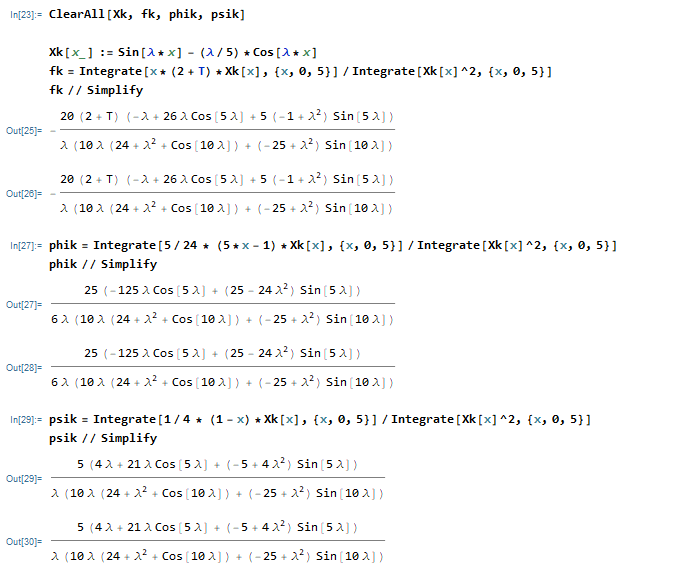
\includegraphics[width=1\linewidth]{image1.png}
\end{figure}
Таким образом, получаем: $$f_k=-\frac{20 (t+2) \left(5 \left(\lambda ^2-1\right) \sin (5 \lambda )-\lambda +26 \lambda  \cos (5 \lambda )\right)}{\lambda  \left(\left(\lambda ^2-25\right) \sin (10 \lambda )+10 \lambda  \left(\lambda ^2+\cos (10 \lambda )+24\right)\right)},$$
$$\varphi_k = \frac{25 \left(\left(25-24 \lambda ^2\right) \sin (5 \lambda )-125 \lambda  \cos (5 \lambda )\right)}{6 \lambda  \left(\left(\lambda ^2-25\right) \sin (10 \lambda )+10 \lambda  \left(\lambda ^2+\cos (10 \lambda )+24\right)\right)},$$
$$\psi_k = \frac{5 \left(\left(4 \lambda_k ^2-5\right) \sin (5 \lambda_k )+4 \lambda_k +21 \lambda_k  \cos (5 \lambda_k )\right)}{\lambda_k  \left(\left(\lambda_k ^2-25\right) \sin (10 \lambda_k )+10 \lambda_k  \left(\lambda_k ^2+\cos (10 \lambda_k )+24\right)\right)}.$$
С помощью полученных коэффициентов составляем следующую задачу Коши:
$$\begin{cases}
    T_k''(t)+\lambda_k^2 T_k(t)=-\frac{20 (t+2) \left(5 \left(\lambda_k ^2-1\right) \sin (5 \lambda_k )-\lambda_k +26 \lambda_k  \cos (5 \lambda_k )\right)}{\lambda_k  \left(\left(\lambda_k ^2-25\right) \sin (10 \lambda_k )+10 \lambda_k  \left(\lambda_k ^2+\cos (10 \lambda_k )+24\right)\right)},\\
    T_k(0)=\frac{25 \left(\left(25-24 \lambda_k ^2\right) \sin (5 \lambda_k )-125 \lambda_k  \cos (5 \lambda_k )\right)}{6 \lambda_k  \left(\left(\lambda_k ^2-25\right) \sin (10 \lambda_k )+10 \lambda_k  \left(\lambda_k ^2+\cos (10 \lambda_k )+24\right)\right)},\\
    T_k'(0)=\frac{5 \left(\left(4 \lambda_k ^2-5\right) \sin (5 \lambda_k )+4 \lambda_k +21 \lambda_k  \cos (5 \lambda_k )\right)}{\lambda_k  \left(\left(\lambda_k ^2-25\right) \sin (10 \lambda_k )+10 \lambda_k  \left(\lambda_k ^2+\cos (10 \lambda_k )+24\right)\right)}.\\
\end{cases}$$
Решим эту задачу. Построим общее однородное решение уравнения рассматриваемой задачи Коши:
$$T_k^{\text{оо}}(t)=A_kcos\lambda_kt+B_ksin\lambda_kt.$$
По виду правой части выпишем частное решение неоднородного уравнения:
$$T_k^{\text{чн}}(t)=C_kt+D_k.$$
Подставим вид частного неоднородного решения в уравнение:
$$C_k \lambda_k^2 t+D_k\lambda_k^2=f_k.$$
Сравнивая соответствующие коэффициенты, получим:
$$\begin{cases}
    C_k = -\frac{20 \left(5 \left(\lambda_k ^2-1\right) \sin (5 \lambda_k )-\lambda_k +26 \lambda_k  \cos (5 \lambda_k )\right)}{\lambda_k^3  \left(\left(\lambda_k ^2-25\right) \sin (10 \lambda_k )+10 \lambda_k  \left(\lambda_k ^2+\cos (10 \lambda_k )+24\right)\right)}, \\
    D_k = -\frac{40\left(5 \left(\lambda_k ^2-1\right) \sin (5 \lambda_k )-\lambda_k +26 \lambda_k  \cos (5 \lambda_k )\right)}{\lambda_k^3  \left(\left(\lambda_k ^2-25\right) \sin (10 \lambda_k )+10 \lambda_k  \left(\lambda_k ^2+\cos (10 \lambda_k )+24\right)\right)}.\\
\end{cases}$$
Тогда получаем общее решение неоднородного уравнения в виде суммы:
$$T_k^{\text{он}}(t)=T_k^{\text{оо}}(t)+T_k^{\text{чн}}(t)=A_kcos\lambda_kt+B_ksin\lambda_kt+C_kt+D_k.$$
Коэффициенты $A_k, B_k$ получим, подставив полученное выражение в начальные условия:
$$\begin{cases}
    T_k(0)=B_k+D_k,\\
    T_k'(0)=C_k-\lambda_kA_k,
\end{cases} \Rightarrow
\begin{cases}
    B_k=\varphi_k-D_k,\\
    A_k = \frac{1}{\lambda_k}(C_k - \psi_k).
\end{cases}$$
Снова прибегнем к помощи Wolfram Mathematica:
\begin{figure}
    \centering
    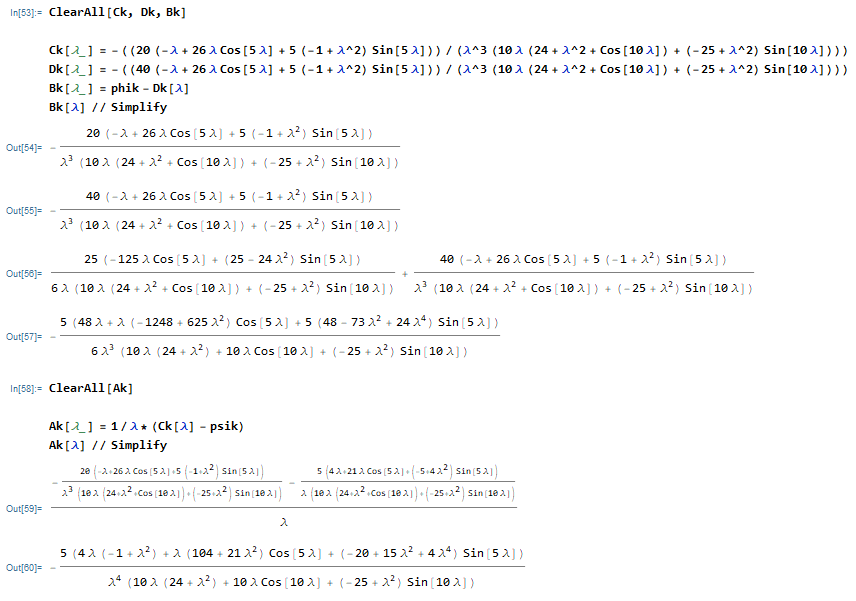
\includegraphics[width=1\linewidth]{image2.png}
\end{figure}
Откуда получаем:
$$\begin{cases}
    A_k=-\frac{5 \left(4 \lambda_k  \left(\lambda_k ^2-1\right)+\lambda_k  \left(21 \lambda_k ^2+104\right) \cos (5 \lambda_k )+\left(4 \lambda_k ^4+15 \lambda_k ^2-20\right) \sin (5 \lambda_k )\right)}{\lambda_k ^4 \left(10 \lambda_k  \left(\lambda_k ^2+24\right)+\left(\lambda_k ^2-25\right) \sin (10 \lambda_k )+10 \lambda_k  \cos (10 \lambda_k )\right)},\\
    B_k=-\frac{5 \left(\left(625 \lambda_k ^2-1248\right) \lambda_k  \cos (5 \lambda_k )+5 \left(24 \lambda_k ^4-73 \lambda_k ^2+48\right) \sin (5 \lambda_k )+48 \lambda_k \right)}{6 \lambda_k ^3 \left(10 \lambda_k  \left(\lambda_k ^2+24\right)+\left(\lambda_k ^2-25\right) \sin (10 \lambda_k )+10 \lambda_k  \cos (10 \lambda_k )\right)}.
\end{cases}$$
Таким образом, из-за излишней громоздкости выражения подставим все найденные коэффициенты мысленно, и тогда мы сможем найти решение задачи для $v$, решение исходной задачи будет иметь вид: $$u(x,t)=\sum^\infty_{k=0}(\sin{\lambda_k x}-\frac{\lambda_k}{5}\cos{\lambda_k x})(A_kcos\lambda_kt+B_ksin\lambda_kt+C_kt+D_k)+\frac{1}{4}(t-\frac{1}{6})x+\frac{1}{4}(\frac{5}{6}-t),$$
где
$$A_k=-\frac{5 \left(4 \lambda_k  \left(\lambda_k ^2-1\right)+\lambda_k  \left(21 \lambda_k ^2+104\right) \cos (5 \lambda_k )+\left(4 \lambda_k ^4+15 \lambda_k ^2-20\right) \sin (5 \lambda_k )\right)}{\lambda_k ^4 \left(10 \lambda_k  \left(\lambda_k ^2+24\right)+\left(\lambda_k ^2-25\right) \sin (10 \lambda_k )+10 \lambda_k  \cos (10 \lambda_k )\right)},$$
$$B_k=-\frac{5 \left(\left(625 \lambda_k ^2-1248\right) \lambda_k  \cos (5 \lambda_k )+5 \left(24 \lambda_k ^4-73 \lambda_k ^2+48\right) \sin (5 \lambda_k )+48 \lambda_k \right)}{6 \lambda_k ^3 \left(10 \lambda_k  \left(\lambda_k ^2+24\right)+\left(\lambda_k ^2-25\right) \sin (10 \lambda_k )+10 \lambda_k  \cos (10 \lambda_k )\right)},$$
$$C_k = -\frac{20 \left(5 \left(\lambda_k ^2-1\right) \sin (5 \lambda_k )-\lambda_k +26 \lambda_k  \cos (5 \lambda_k )\right)}{\lambda_k^3  \left(\left(\lambda_k ^2-25\right) \sin (10 \lambda_k )+10 \lambda_k  \left(\lambda_k ^2+\cos (10 \lambda_k )+24\right)\right)},$$
$$D_k = -\frac{40\left(5 \left(\lambda_k ^2-1\right) \sin (5 \lambda_k )-\lambda_k +26 \lambda_k  \cos (5 \lambda_k )\right)}{\lambda_k^3  \left(\left(\lambda_k ^2-25\right) \sin (10 \lambda_k )+10 \lambda_k  \left(\lambda_k ^2+\cos (10 \lambda_k )+24\right)\right)},$$
$\lambda_k$ найдем при визуализации из уравнения $\tg{5\lambda_k}=\frac{\lambda_k}{5}.$ 
\subsubsection*{Визуализация решения}
Для визуализации необходимо перенести полученное аналитически решение в Wolfram Mathematica, а так же вычислить недостающий на данном этапе элемент, а имеено собственные значения $\lambda_k$:
\begin{figure}
    \centering
    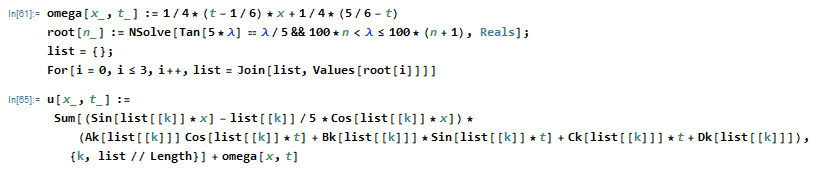
\includegraphics[width=1\linewidth]{image3.png}
\end{figure}
Теперь построим две визуализации для нашей задачи:
\begin{enumerate}
    \item Профиля струны во времени для конкретного момента времени с возможностью
изменения:
        \begin{figure}
            \centering
            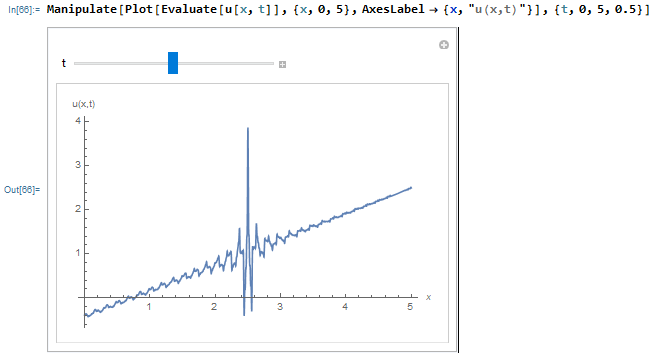
\includegraphics[width=1\linewidth]{image6.png}
        \end{figure}
    \item Профиля струны во времени на всем промежутке времени:
    \begin{figure}
        \centering
        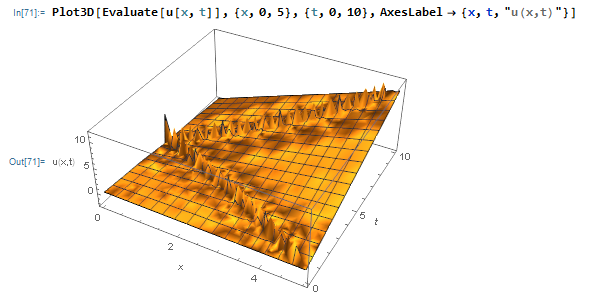
\includegraphics[width=1\linewidth]{image7.png}
    \end{figure}
\end{enumerate}

\newpage
\section*{Задача 2}
\subsubsection*{Получение решения}
Перепишем условие задачи:
$$\begin{cases}
    u_{tt}=\Delta u,\\
    u|_{x=0}=u_x|_{x=5}=0,\\
    u_y|_{y=0}=u|_{y=9}=0,\\
    u|_{t=0} = e^{x+y},\\
    u_t|_{t=0}=e^{x-y}.\\
\end{cases}$$
Решение задачи будем искать в виде:
$$u(x,y,t)=T(t)V(x,y),$$
подставим данное представление в уравнение нашей задачи, тогда получим:
$$T''(t)V(x,y)=\Delta V(x,y) T(t),$$
разделим обе части уравнения на $T(t)V(x,y)$, тогда получим:
$$\frac{T''}{T}=\frac{\Delta V}{V}=-\lambda^2.$$
Отсюда составим задачу для $V(x,y)$:
$$\begin{cases}
    \Delta V+\lambda^2 V=0, \\
    V|_{x=0}=V_x|_{x=5}=0,\\
    V_y|_{y=0}=V|_{y=9}=0.\\
\end{cases}$$
Получившуюся задачу будем решать с помощью замены: $$V(x,t)=X(x)Y(y),$$
подставим в уравнение рассматриваемой задачи и получим: $$\frac{YX''+XY''}{XY}=-\lambda^2 \Rightarrow \frac{X''}{X}+\frac{Y''}{Y}=-\lambda^2 \Rightarrow \frac{X''}{X}=-\frac{Y''}{Y}-\lambda^2=-\mu^2.$$
Тогда получим два уравнения:
$$X''+\mu^2X=0,\\$$ $$Y''+\nu^2Y=0,$$
где $\nu^2=\lambda^2-\mu^2.$ Воспользуемся граничными условиями исходной задачи и построим две задачи Штурма-Лиувилля:
$$\begin{cases}
    X''+\mu^2X=0,\\
    X(0)=0,\\
    X'(5)=0,
\end{cases}
\begin{cases}
    Y''+\nu^2Y=0,\\
    Y(9)=0,\\
    Y'(0)=0.
\end{cases}$$
Рассмотрим задачу для $X(x)$. Из уравнения имеем общее решение:
$$X(x)=A\cos{\mu x}+B\sin{\mu x},$$
подставим в граничные условия:
$$\begin{cases}
    X(0)=A=0,\\
    X'(5)=\mu B\cos{5\mu},
\end{cases}\Rightarrow 
\cos{5\mu}=0 \Rightarrow \mu_n=\dfrac15 (\frac{\pi}{2}+\pi n), n=1, 2, ...$$
Таким образом, решение задачи Штурма-Лиувилля для $X(x)$ имеет вид:
$$X_n(x)=\sin{x\mu_n}, \mu_n=\dfrac15 (\frac{\pi}{2}+\pi n), n=1, 2, ...$$
Решим теперь вторую задачу, для $Y(y)$:
$$Y(y)=A\cos{\nu y}+B\sin{\nu y},$$
$$\begin{cases}
    Y'(0)=B\nu=0, \Rightarrow B=0,\\
    Y(9)=A\cos{9\nu}=0, 
\end{cases}\Rightarrow \nu_m=\dfrac19 (\frac{\pi}{2}+\pi m), m=1,2,...$$
Таким образом, решение данной задачи Штурма-Лиувилля имеет вид:
 $$Y_m(y)=\cos{y\nu_m}, \nu_m=\dfrac19 (\frac{\pi}{2}+\pi m), m=1,2,...$$
 Тогда решение исходной задачи примет вид:
 $$u(x,y,t)=\sum_{n,m=1}^\infty T_{nm}(t)\sin{x\mu_n}\cos{y\nu_m}.$$
 Подставим в исходную задачу:
 $$\begin{cases}
    \sum_{n,m=1}^\infty T_{nm}''(t)\sin{x\mu_n}\cos{y\nu_m}+\sum_{n,m=1}^\infty T_{nm}(t)(\mu_n^2 \sin{x\mu_n}\cos{y\nu_m}+\nu_m^2\sin{x\mu_n}\cos{y\nu_m})=0,\\
    \sum_{n,m=1}^\infty T_{nm}(0)\sin{x\mu_n}\cos{y\nu_m}=e^{x+y},\\
    \sum_{n,m=1}^\infty T_{nm}'(0)\sin{x\mu_n}\cos{y\nu_m}=e^{x-y}.
\end{cases}$$
Заметим, что уравнение полученной задачи можно переписать в виде:
$$\sum_{n,m=1}^\infty T_{nm}''(t)\sin{x\mu_n}+\sum_{n,m=1}^\infty T_{nm}(t)(\mu_n^2 +\nu_m^2)=0, \Rightarrow T_{nm}''(t)+\lambda_{nm}^2T_{nm}(t)=0, \Rightarrow $$
$$\Rightarrow T_{nm}(t)=A_{nm}\cos{\lambda_{nm}t}+B_{nm}\sin{\lambda_{nm}t}.$$
Тогда, подставляя в начальные условия, получим:
$$\begin{cases}
    \sum_{n,m=1}^\infty A_{nm}\sin{x\mu_n}\cos{y\nu_m}=e^{x+y},\\
    \sum_{n,m=1}^\infty \lambda_{nm}B_{nm}\sin{x\mu_n}\cos{y\nu_m}=e^{x-y}.
\end{cases}$$
Разложим наши функции $\varphi(x,y)=e^{x+y}, \psi(x,y)=e^{x-y}$ в ряд Фурье по собственным функциям:
$$A_{nm}=\frac{\int_0^5\int_0^9e^{x+y}\sin{x\mu_n}\cos{y\nu_m}dy dx}{\int_0^5\int_0^9(\sin{x\mu_n}\cos{y\nu_m})^2dy dx}=[\text{переобозначим}]=\frac{1}{I}\int_0^5 e^x\sin{x\mu_n}\int_0^9 e^y\cos{y\nu_m}dydx,$$
$$B_{nm}=\frac{1}{I}\int_0^5\int_0^9e^{x-y}\sin{x\mu_n}\cos{y\nu_m}dy dx=\frac{1}{I}\int_0^5 e^x\sin{x\mu_n}\int_0^9 \frac{1}{e^y}\cos{y\nu_m}dydx.$$
Посчитаем отдельно каждый из интегралов:
$$I=\int_0^5\int_0^9(\sin{x\mu_n}\cos{y\nu_m})^2dy dx=\int_0^5\sin^2{x\mu_n}\int_0^9\cos^2{y\nu_m}dy dx=\int_0^5\frac{1-\cos{2y\mu_n}}{2}\int_0^9\frac{1+\cos{2y\nu_m}}{2}dy dx=$$
$$=\frac{9+\frac{1}{2\nu_m}\sin{18\nu_m}}{2}\int_0^5\frac{1-\cos{2y\mu_n}}{2}dx=\frac{9+\frac{1}{2\nu_m}\sin{18\nu_m}}{2}\frac{5-\frac{1}{2\mu_n}\sin{18\mu_n}}{2}=[\text{подставим значения}]=\frac{45}{4}$$
$$I_1=\int_0^9e^{y}\cos{y\nu_m}dy=[\text{решаем по частям}]=\left[u=e^y \Rightarrow du=e^y dy, dv=\cos{y\nu_m}dy \Rightarrow v=\frac{1}{\nu_m}\sin{y\nu_m} \right]=$$
$$=\frac{1}{\nu_m}\sin{y\nu_m}\cdot e^y |_{y=0}^{y=9}-\frac{1}{\nu_m}\int_0^9e^y\sin{y\nu_m}dy=\frac{1}{\nu_m}(\sin{9\nu_m}\cdot e^9-\int_0^9e^y\sin{y\nu_m}dy)=[\text{снова по частям}]=$$
$$=\frac{1}{\nu_m}(e^9(\sin{9\nu_m}+\frac{1}{\nu_m}\cos{9\nu_m})-\frac{1}{\nu_m}-\frac{1}{\nu_m}\int_0^9e^y\cos{\nu_my}dy), \Rightarrow \nu_m I_1+\frac{1}{\nu_m}I_1=e^9(\sin{9\nu_m}+\frac{1}{\nu_m}\cos{9\nu_m})-\frac{1}{\nu_m}, $$
$$\Rightarrow (\frac{\nu_m^2+1}{\nu_m})I_1=e^9(\sin{9\nu_m}+\frac{1}{\nu_m}\cos{9\nu_m})-\frac{1}{\nu_m},\Rightarrow I_1=\frac{1}{1+\nu_m^2}(e^9(\nu_m\sin{9\nu_m}+\cos{9\nu_m})-1)=$$
$$=[\text{частично подставим значение $\nu_m$}]=\frac{1}{1+\nu_m^2}((-1)^me^9-1)$$
$$I_2=\int_0^5 e^x\sin{x\mu_n}dx=[\text{аналогично $I_1$}]=\frac{1}{1+\mu_n^2}(1-(-1)^ne^5)$$
$$I_3=\int_0^9 \frac{1}{e^y}\cos{y\nu_m}dy=[\text{аналогично $I_1$}]=\frac{1}{1+\nu_m^2}((-1)^m\frac{1}{e^5}-1)$$
$$I_4=I_2=\frac{1}{1+\mu_n^2}(1-(-1)^ne^5).$$
Таким образом, получаем:
$$A_{nm}=\frac{4}{45}\cdot\frac{1}{1+\nu_m^2}((-1)^me^9-1)\cdot\frac{1}{1+\mu_n^2}(1-(-1)^ne^5)=\frac{4}{45}\cdot\frac{1}{(1+\nu_m^2)(1+\mu_n^2)}((-1)^me^9-1)((1-(-1)^ne^5)),$$
$$B_{nm}=\frac{4}{45}\cdot\frac{1}{1+\nu_m^2}((-1)^m\frac{1}{e^5}-1)\cdot\frac{1}{1+\mu_n^2}(1-(-1)^ne^5)=\frac{4}{45}\cdot\frac{1}{(1+\nu_m^2)(1+\mu_n^2)}((-1)^m\frac{1}{e^5}-1)(1-(-1)^ne^5).$$
Итого, мысленно подставив полученные коэффициенты в решение уравнения рассматриваемой задачи, получим решение рассматриваемой задачи Коши:
$$T_{nm}(t)=A_{nm}\cos{\lambda_{nm}t}+B_{nm}\sin{\lambda_{nm}t},$$
где $$\lambda_{nm}^2=\nu_m^2+\mu_n^2=(\dfrac19 (\frac{\pi}{2}+\pi m))^2+(\dfrac15 (\frac{\pi}{2}+\pi n))^2.$$
Итого, решение исходной задачи представимо в виде:
$$u(x,y,t)=\sum_{n,m=1}^\infty (A_{nm}\cos{\lambda_{nm}t}+B_{nm}\sin{\lambda_{nm}t})\sin{x\mu_n}\cos{y\nu_m},$$
где 
$$A_{nm}=\frac{4}{45}\cdot\frac{1}{(1+\nu_m^2)(1+\mu_n^2)}((-1)^me^9-1)((1-(-1)^ne^5)),$$
$$B_{nm}=\frac{4}{45}\cdot\frac{1}{(1+\nu_m^2)(1+\mu_n^2)}((-1)^m\frac{1}{e^5}-1)(1-(-1)^ne^5),$$
$$\mu_n=\dfrac15 (\frac{\pi}{2}+\pi n), n=1, 2, ...,\   \nu_m=\dfrac19 (\frac{\pi}{2}+\pi m), m=1,2,...,$$
$$\lambda_{nm}=\sqrt{\mu_n^2+\nu_m^2}$$
\subsubsection*{Визуализация решения}
Перенесём полученное ранее аналитическое решение в Wolfram Mathematica:
\begin{figure}
    \centering
    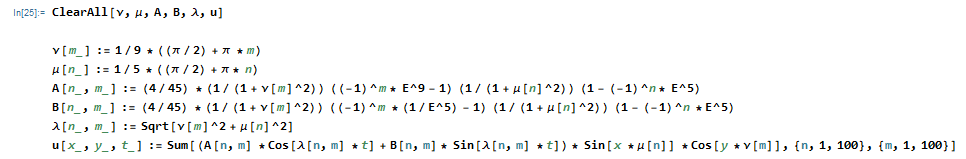
\includegraphics[width=1\linewidth]{image4.png}
\end{figure}
После этого строим визуализацию прямоугольного контура во времени для конкретного
времени с возможностью изменения:
\begin{figure}
    \centering
    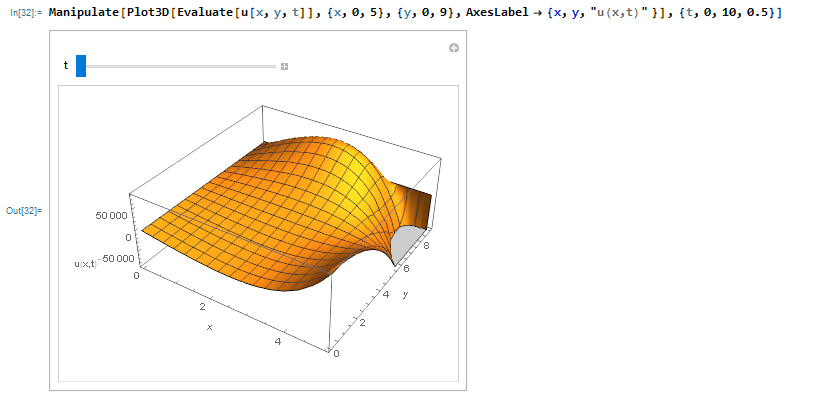
\includegraphics[width=1\linewidth]{image5.png}
\end{figure}
\end{document}
